
% vim: set ft=tex tabstop=4 shiftwidth=4 noexpandtab:

% opening %{{{1

\documentclass[tikz, border=1mm]{standalone}

% packages and libraries %{{{1

% ---- not necessary since the documentclass[tikz ...] requires it automatically
% \usepackage{tikz}

\usetikzlibrary{calc,intersections,angles,quotes,shapes.geometric}

\usepackage{amsmath}

\usepackage{tkz-euclide}


% opening %{{{1

\begin{document}
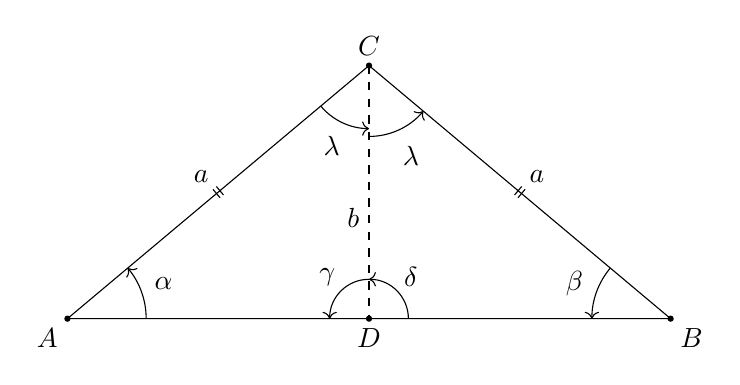
\begin{tikzpicture}[scale=1.0]

% parameters %{{{1

	\def\len{5}
	\def\ang{40}

% coordinates %{{{1

	\coordinate (A) at (0,0);
	\coordinate (B) at (0:{2*\len*cos(\ang)});
	\coordinate (C) at (\ang:\len);

	\coordinate (D) at (0:{\len*cos(\ang)});

% points, dots, vertices %{{{1

	\fill (A) circle (0.4mm);
	\fill (B) circle (0.4mm);
	\fill (C) circle (0.4mm);
	\fill (D) circle (0.4mm);

% triangle %{{{1

	\draw (A) -- (B) -- (C) -- cycle;
	\draw[dashed] (C) -- (D);

% points, dots, vertices labels %{{{1

	\node[below left] at (A) {$A$};
	\node[below right] at (B) {$B$};
	\node[above] at (C) {$C$};
	\node[below] at (D) {$D$};

% segment labels %{{{1

	\node[above left]  at ($(A)!0.5!(C)$) {$a$};
	\node[above right] at ($(B)!0.5!(C)$) {$a$};

	\node[left]  at ($(C)!0.6!(D)$) {$b$};

% segments, sides marks %{{{1

	\tkzMarkSegments[mark=||, size=2pt](A,C)
	\tkzMarkSegments[mark=||, size=2pt](B,C)

% 	\tkzMarkSegments[mark=|, size=2pt](A,D)
% 	\tkzMarkSegments[mark=|, size=2pt](D,B)

% angles labels %{{{1

	\pic[draw, ->, "$\alpha$", angle radius=1.0cm, angle eccentricity=1.3]
	{angle = D--A--C};

	\pic[draw, ->, "$\beta$", angle radius=1.0cm, angle eccentricity=1.3]
	{angle = C--B--D};

	\pic[draw, ->, "$\gamma$", angle radius=0.5cm, angle eccentricity=1.5]
	{angle = C--D--A};

	\pic[draw, ->, "$\delta$", angle radius=0.5cm, angle eccentricity=1.5]
	{angle = B--D--C};

	\pic[draw, ->, "$\lambda$", angle radius=0.8cm, angle eccentricity=1.4]
	{angle = A--C--D};

	\pic[draw, ->, "$\lambda$", angle radius=0.9cm, angle eccentricity=1.4]
	{angle = D--C--B};

% closing %{{{1

\end{tikzpicture}
\end{document}
